\documentclass[border=8pt]{standalone}
\usepackage[T1]{fontenc}
\usepackage{mathptmx}
\usepackage{tikz}
\usetikzlibrary{arrows.meta,positioning,fit,calc,shapes.geometric,shapes.misc,shapes.multipart,backgrounds}
\tikzset{
  arr/.style={-{Stealth[length=2.4mm,width=1.8mm]},line width=0.6pt},
  box/.style={draw,line width=0.6pt,align=center,rounded corners=2pt},
}

\begin{document}
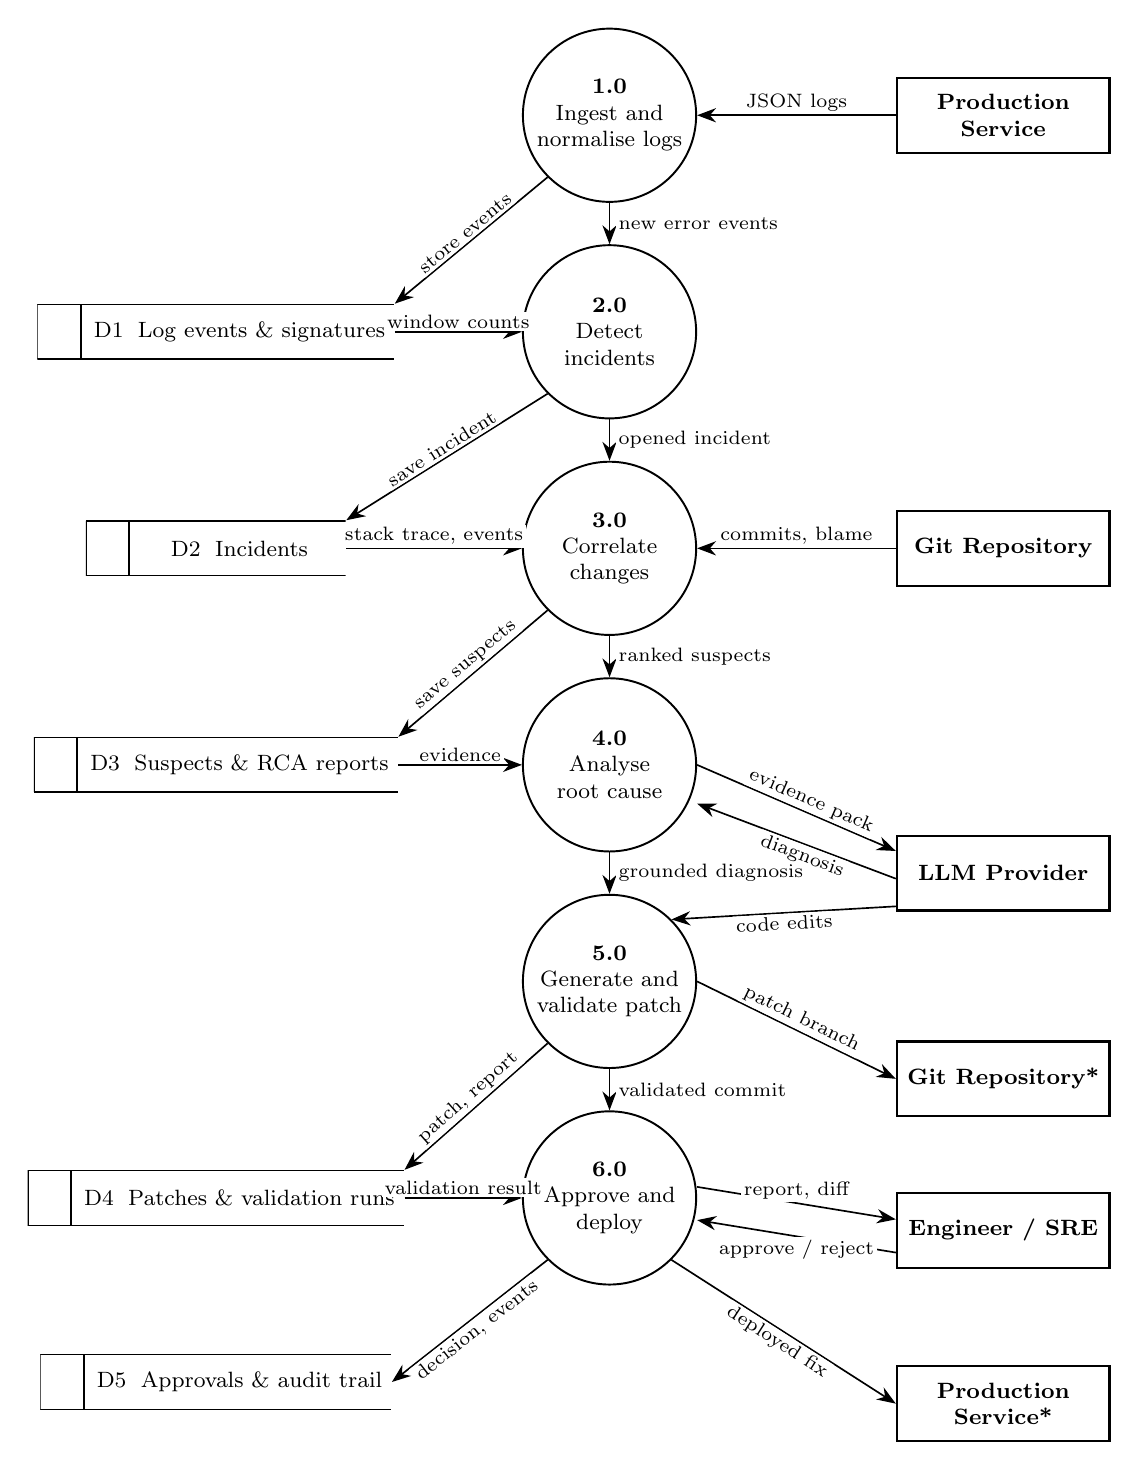
\begin{tikzpicture}[font=\small,
  proc/.style={circle, draw, line width=0.7pt, minimum size=2.2cm, align=center, inner sep=1pt, font=\footnotesize},
  ent/.style={draw, line width=0.8pt, minimum width=2.7cm, minimum height=0.95cm, align=center, font=\footnotesize\bfseries},
  store/.style={draw=none, minimum width=3.3cm, minimum height=0.7cm, align=left, font=\footnotesize, path picture={
     \draw[line width=0.7pt] (path picture bounding box.north west) -- (path picture bounding box.north east);
     \draw[line width=0.7pt] (path picture bounding box.south west) -- (path picture bounding box.south east);
     \draw[line width=0.7pt] (path picture bounding box.north west) -- (path picture bounding box.south west);
     \draw[line width=0.7pt] ([xshift=0.55cm]path picture bounding box.north west) -- ([xshift=0.55cm]path picture bounding box.south west);}},
  lab/.style={font=\scriptsize, fill=white, inner sep=1pt, align=center}]
\def\dy{2.75}
\node[proc] (p1) at (0,0) {\textbf{1.0}\\ Ingest and\\ normalise logs};
\node[proc] (p2) at (0,-\dy) {\textbf{2.0}\\ Detect\\ incidents};
\node[proc] (p3) at (0,-2*\dy) {\textbf{3.0}\\ Correlate\\ changes};
\node[proc] (p4) at (0,-3*\dy) {\textbf{4.0}\\ Analyse\\ root cause};
\node[proc] (p5) at (0,-4*\dy) {\textbf{5.0}\\ Generate and\\ validate patch};
\node[proc] (p6) at (0,-5*\dy) {\textbf{6.0}\\ Approve and\\ deploy};
\node[store] (d1) at (-5.0,-1*\dy) {\hspace{0.55cm}\,D1\; Log events \& signatures};
\node[store] (d2) at (-5.0,-2*\dy) {\hspace{0.55cm}\,D2\; Incidents};
\node[store] (d3) at (-5.0,-3*\dy) {\hspace{0.55cm}\,D3\; Suspects \& RCA reports};
\node[store] (d4) at (-5.0,-5*\dy) {\hspace{0.55cm}\,D4\; Patches \& validation runs};
\node[store] (d5) at (-5.0,-5.85*\dy) {\hspace{0.55cm}\,D5\; Approvals \& audit trail};
\node[ent] (prod) at (5.0,0) {Production\\ Service};
\node[ent] (git) at (5.0,-2*\dy) {Git Repository};
\node[ent] (llm) at (5.0,-3.5*\dy) {LLM Provider};
\node[ent] (git2) at (5.0,-4.45*\dy) {Git Repository*};
\node[ent] (eng) at (5.0,-5.15*\dy) {Engineer / SRE};
\node[ent] (prod2) at (5.0,-5.95*\dy) {Production\\ Service*};
% main flow
\draw[arr] (p1) -- node[lab, right=2pt] {new error events} (p2);
\draw[arr] (p2) -- node[lab, right=2pt] {opened incident} (p3);
\draw[arr] (p3) -- node[lab, right=2pt] {ranked suspects} (p4);
\draw[arr] (p4) -- node[lab, right=2pt] {grounded diagnosis} (p5);
\draw[arr] (p5) -- node[lab, right=2pt] {validated commit} (p6);
% stores: written by the process above, read by the process alongside
\draw[arr] (p1.south west) -- node[lab, sloped, above] {store events} (d1.north east);
\draw[arr] (d1.east) -- node[lab, above] {window counts} (p2.west);
\draw[arr] (p2.south west) -- node[lab, sloped, above] {save incident} (d2.north east);
\draw[arr] (d2.east) -- node[lab, above] {stack trace, events} (p3.west);
\draw[arr] (p3.south west) -- node[lab, sloped, above] {save suspects} (d3.north east);
\draw[arr] (d3.east) -- node[lab, above] {evidence} (p4.west);
\draw[arr] (p5.south west) -- node[lab, sloped, above] {patch, report} (d4.north east);
\draw[arr] (d4.east) -- node[lab, above] {validation result} (p6.west);
\draw[arr] (p6.south west) -- node[lab, sloped, below] {decision, events} (d5.east);
% entities
\draw[arr] (prod) -- node[lab, above] {JSON logs} (p1);
\draw[arr] (git) -- node[lab, above] {commits, blame} (p3);
\draw[arr] (p4.east) -- node[lab, sloped, above, pos=0.55] {evidence pack} ([yshift=8pt]llm.west);
\draw[arr] ([yshift=-2pt]llm.west) -- node[lab, sloped, below, pos=0.45] {diagnosis} ([yshift=-14pt]p4.east);
\draw[arr] ([yshift=-12pt]llm.west) -- node[lab, sloped, below] {code edits} (p5.north east);
\draw[arr] (p5.east) -- node[lab, sloped, above] {patch branch} (git2.west);
\draw[arr] ([yshift=4pt]p6.east) -- node[lab, above] {report, diff} ([yshift=4pt]eng.west);
\draw[arr] ([yshift=-8pt]eng.west) -- node[lab, below] {approve / reject} ([yshift=-8pt]p6.east);
\draw[arr] (p6.south east) -- node[lab, sloped, below] {deployed fix} (prod2.west);
\end{tikzpicture}
\end{document}
